\documentclass[11pt,a4paper]{article}
\usepackage[T1]{fontenc}
\usepackage[utf8]{inputenc}
\usepackage{lmodern}
\usepackage[margin=2.1cm]{geometry}
\usepackage{microtype}
\usepackage{xcolor}
\usepackage{tabularx,booktabs,array}
\usepackage{enumitem}
\usepackage{titlesec}
\usepackage{tikz}
\usetikzlibrary{arrows.meta,positioning,calc}
\usepackage[most]{tcolorbox}
\usepackage{fancyhdr}
\usepackage[hidelinks]{hyperref}

\definecolor{navy}{HTML}{14213D}
\definecolor{accent}{HTML}{C4571F}
\definecolor{llmfill}{HTML}{E4EAF6}
\definecolor{llmline}{HTML}{2F4A85}
\definecolor{codefill}{HTML}{ECEAE4}
\definecolor{codeline}{HTML}{8A8578}
\definecolor{humfill}{HTML}{E2F0E6}
\definecolor{humline}{HTML}{2F7A4A}
\definecolor{okc}{HTML}{2F7A4A}
\definecolor{wipc}{HTML}{9A6A00}
\definecolor{badc}{HTML}{B3401A}

\titleformat{\section}{\Large\bfseries\color{navy}}{\thesection}{0.6em}{}
\titleformat{\subsection}{\large\bfseries\color{navy}}{\thesubsection}{0.6em}{}
\titlespacing*{\section}{0pt}{1.2em}{0.5em}
\setlength{\parindent}{0pt}
\setlength{\parskip}{0.5em}
\setlist{itemsep=0.15em,topsep=0.25em}
\renewcommand{\arraystretch}{1.25}
\newcolumntype{L}[1]{>{\raggedright\arraybackslash}p{#1}}
\newcolumntype{Y}{>{\raggedright\arraybackslash}X}
\newcommand{\decision}[1]{\textbf{\color{accent}[Decision #1]}}
\newcommand{\ok}[1]{\textcolor{okc}{\textbf{#1}}}
\newcommand{\wip}[1]{\textcolor{wipc}{\textbf{#1}}}
\newcommand{\bad}[1]{\textcolor{badc}{\textbf{#1}}}

\newtcolorbox{keybox}{colback=navy!4,colframe=navy,boxrule=0.6pt,arc=2pt,left=8pt,right=8pt,top=6pt,bottom=6pt}
\newtcolorbox{rulebox}{colback=accent!5,colframe=accent,boxrule=0.6pt,arc=2pt,left=8pt,right=8pt,top=6pt,bottom=6pt}

\pagestyle{fancy}
\fancyhf{}
\renewcommand{\headrulewidth}{0pt}
\fancyfoot[L]{\footnotesize\color{gray}Security, Augmented \textperiodcentered{} shared direction v2}
\fancyfoot[R]{\footnotesize\color{gray}\thepage}

\begin{document}

{\color{navy}\Huge\bfseries Security, Augmented: one shared direction\par}
\vspace{0.3em}
{\Large Merging the perception prototype and the agent layer into one system\par}
\vspace{0.3em}
{\color{gray}Alignment note for the group \textperiodcentered{} v2, 25 November 2026 \textperiodcentered{} for the meeting on Friday, before the 2 December check-in\par}
\vspace{0.8em}

\begin{keybox}
\textbf{In one sentence.} A cheap trigger finds the moments worth a look; a general eye describes what
happened, with the frames to prove it; an agent checks it against what the site knows and explains why it
matters; a person decides, and every step is logged.
\end{keybox}

\section{Why this note}
Guards are flooded with false alarms: monitoring centres report that about half of their alarms are false,
and one US guarding firm cut its daily alerts by 62\,\% after adding AI filtering.\footnote{Calipsa survey of
monitoring centres (2020); Milestone and Genesis Security case study. Taken from the agent-layer check-in of
25 November.} Our goal is a system that does this filtering with the judgement of an experienced guard, on any
site, while the guard keeps every decision.

Two of us explored the problem from opposite ends. The \textbf{perception prototype} (Gemini on CAVIAR) asked:
\emph{can a model describe everything that happens in a video, and prove it?} The \textbf{agent layer}
(Claude on a replayed MEVA site, branch \texttt{cctv-playground}) asked: \emph{given an alert, can an agent decide
whether a person needs to see it?} The answers fit together. This note merges them into one target, one way to
test it and one list of decisions. It adds no new work; it orders what we already plan.

\section{Where we are}

\begin{center}
\small
\begin{tabularx}{\textwidth}{L{2.6cm}YY}
\toprule
& \textbf{Perception prototype} & \textbf{Agent layer (\texttt{cctv-playground})}\\
\midrule
Footage & CAVIAR: 16 clips, one lobby and one shopping corridor, actors & MEVA: 7 cameras, 14 min of a closed Sunday, 17 alerts (10 real, 7 look-alikes); CAUCAFall for falls\\
What it does & Describes the whole video in 10\,s windows, verifies with a second look, writes a guard report where every claim cites frames & Detector alert $\rightarrow$ triage agent with badge log, roster, procedures and neighbouring cameras $\rightarrow$ video check $\rightarrow$ rules in code $\rightarrow$ guard approves $\rightarrow$ report draft $\rightarrow$ audit log\\
Model & Gemini 3.6 Flash, thinking High & Claude Haiku 5.5 (16 frames); Sonnet 5.5 for objects or empty answers\\
Best result & 126/126 valid citations; falls on never-seen clips 3/3 & 14/17 verdicts right in every run; 10/10 real events kept; 0 falls missed\\
Time to alert & median 63\,s (dev) and 135\,s (never seen) & median 22--25\,s, including the stand-in detector's delay\\
Cost & $\approx$\$8.5--8.9k per camera per month (all footage analysed) & $\approx$\$0.01 per alert; $\approx$\$2.50--7 per camera per month if 2\,\% of footage is checked (assumption)\\
Main gap & No site knowledge, so no alert sorting (reduction 0\,\% / 20\,\%); slow; expensive & Detector is a stand-in that knows the labels; one site, daytime; this site cannot show alert reduction (10 of 17 alerts are real)\\
\bottomrule
\end{tabularx}
\end{center}

\textbf{What both explorations found independently}
\begin{itemize}
\item \textbf{Objects are the hard case, falls are not.} Every model found every fall. A bag hidden behind a
chair was missed on CAVIAR, and on MEVA only Sonnet found the abandoned bag (6 of 6 runs; Haiku and every Gemini
setting tested: 0 of 3).
\item \textbf{The second look must use new evidence.} On CAVIAR a false fall was confirmed because verification
re-read the same text. On MEVA a cheap check plus a targeted second look on new frames scored 94\,\%, against
81\,\% for a majority vote: the models share blind spots, so voting throws the right answer away.
\item \textbf{Safety rules belong in code.} The agent named every fall look-alike correctly; the rule still sent
each one to a person, which is what we want.
\item \textbf{Site records matter as much as the model.} The roster and badge log explained the guard's car and
the cleaners. Without them, the perception prototype could only describe.
\item \textbf{Image limits.} Small people (about 27\,px tall on CAVIAR) are the limit, not blur. Thinking High
added no accuracy over Low in the model comparison.
\end{itemize}

\section{Target system}

\begin{center}
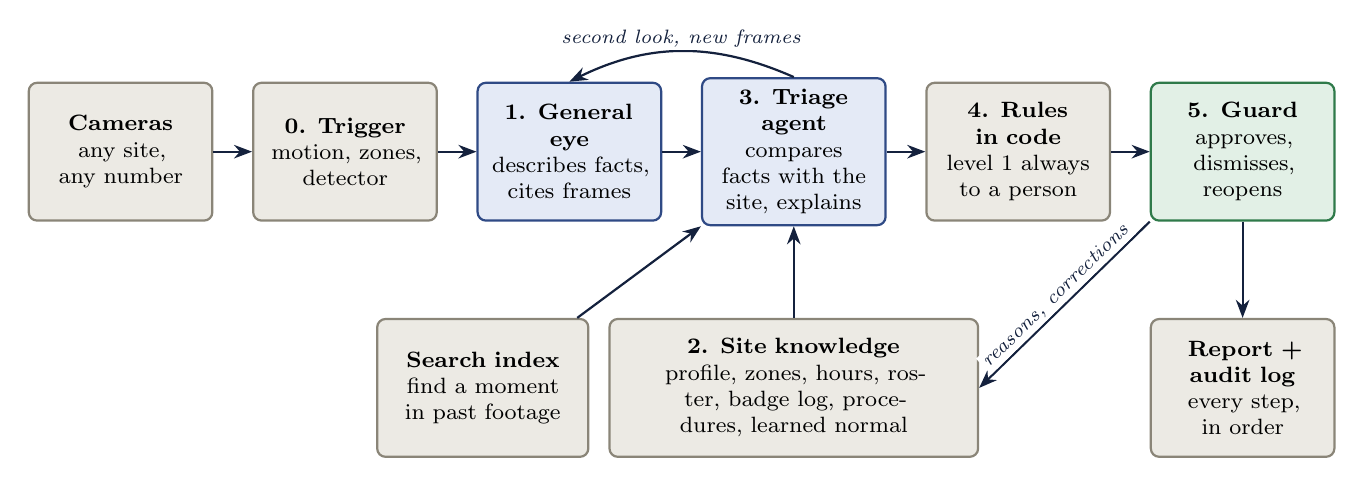
\begin{tikzpicture}[
  font=\footnotesize,
  box/.style={draw,rounded corners=3pt,thick,align=center,inner sep=4pt,text width=2.05cm,minimum height=1.75cm},
  llm/.style={box,fill=llmfill,draw=llmline},
  code/.style={box,fill=codefill,draw=codeline},
  hum/.style={box,fill=humfill,draw=humline},
  arr/.style={-{Stealth[length=2.3mm]},thick,draw=navy},
  lab/.style={font=\scriptsize\itshape,text=navy,fill=white,inner sep=1pt}
]
\node[code] (cam)    at (0,0)     {\textbf{Cameras}\\any site,\\any number};
\node[code] (trig)   at (2.85,0)  {\textbf{0. Trigger}\\motion, zones, detector};
\node[llm]  (eye)    at (5.7,0)   {\textbf{1. General\\eye}\\describes facts, cites frames};
\node[llm]  (agent)  at (8.55,0)  {\textbf{3. Triage\\agent}\\compares facts with the site, explains};
\node[code] (rules)  at (11.4,0)  {\textbf{4. Rules in code}\\level 1 always to a person};
\node[hum]  (guard)  at (14.25,0) {\textbf{5. Guard}\\approves, dismisses, reopens};
\node[code,text width=4.4cm] (site) at (8.55,-3.0) {\textbf{2. Site knowledge}\\profile, zones, hours, roster, badge log, procedures, learned normal};
\node[code,text width=2.4cm] (search) at (4.6,-3.0) {\textbf{Search index}\\find a moment in past footage};
\node[code,text width=2.05cm] (log) at (14.25,-3.0) {\textbf{Report + audit log}\\every step, in order};
\draw[arr] (cam) -- (trig);
\draw[arr] (trig) -- (eye);
\draw[arr] (eye) -- (agent);
\draw[arr] (agent) -- (rules);
\draw[arr] (rules) -- (guard);
\draw[arr] (site) -- (agent);
\draw[arr] (search) -- (agent.south west);
\draw[arr] (agent.north) to[bend right=25] node[lab,above]{second look, new frames} (eye.north);
\draw[arr] (guard) -- (log);
\draw[arr] (guard.south west) -- node[lab,sloped,above]{reasons, corrections} (site.east);
\end{tikzpicture}
\end{center}
{\footnotesize\color{gray}Blue: language model. Grey: code and data. Green: human.}

\textbf{0. Trigger (code).} Cheap motion and zone checks, then the detector, decide \emph{when} to look, never
\emph{what} happened. This is what brings cost from thousands of dollars per camera per month to a few dollars,
and time to alert under 30\,s. A trigger can miss events, so its misses must be measured on real detections, not
on the stand-in used so far. Level-1 zones (exits, stairwells) can also be sampled at a fixed rate whatever the
trigger says.

\textbf{1. General eye (vision model, the same for every site).} Describes facts in an open vocabulary: people,
postures, objects, movement, physical contact, smoke, light. It never names a crime: a fight is \emph{``two people
in physical contact, one falls, three others move away quickly''}. It works as a cascade: a cheap first look, then
a stronger model on new frames for objects, empty answers or doubtful cases; for a person on the floor, a neutral
close look over about 20 frames. Each claim cites its frames.

\textbf{2. Site knowledge (changes for each site).} What an experienced guard knows: the site profile
(Section~5), the site's own records (roster, badge log, procedures with priorities), optionally the normal activity
learned from ordinary footage, and the reasons the guard gave when dismissing earlier alerts.

\textbf{3. Triage agent (the intelligence).} Compares what is seen with what is expected here, uses tools
(site records, neighbouring cameras, the search index), links the same event across neighbouring cameras, and
gives a verdict: \emph{send to a person}, \emph{dismiss with a reason}, or \emph{needs review}. It explains in one
or two sentences and cites the rule it applied. Example: \emph{``Person in the loading bay at 02:10. The bay is
closed at night and no delivery is planned (procedure 1). Send.''} The same facts on another site can give a
different answer.

\textbf{4. Rules in code.} A possible fall, fire or act of violence always reaches a person, whatever the agent
concludes; any tool failure escalates. The agent's view is shown, not used to hide a level-1 event.

\textbf{5. Guard, report and audit log.} The guard approves, dismisses with a reason, or reopens. Actions are
simulated; the system contacts no one. Code writes the facts of the report (times, cameras, action) and the model
writes the prose; both are checked. Every verdict, decision, action and report goes into the audit log.

\textbf{Anonymous tracking.} To tell a story (\emph{``P3 put the bag down at 00:41 and left at 00:58''}), each
person gets a pseudonym that follows them inside one camera's footage, from appearance and movement only. Linking
across neighbouring cameras is done today for vehicles (the red pickup seen on two cameras); for people it needs a
group decision. Even anonymous, tracking is personal data under the nLPD and goes into the privacy note.

\begin{rulebox}
\textbf{Rules that stay true everywhere}
\begin{description}[leftmargin=2.2em,labelwidth=1.8em,font=\bfseries\color{accent}]
\item[R1.] Facts are descriptive and cite their frames. Interpretation is shown as the system's view, with
its doubts, never as a fact.
\item[R2.] A person decides. The system ranks and explains; actions are simulated and it contacts no one.
\item[R3.] Level-1 events are always shown, even if the agent or the site profile says they are normal.
\item[R4.] What was not analysed is reported, so silence never means ``nothing happened''.
\item[R5.] No identification of people: no faces, no gait, no re-identification across videos; faces are blurred
in report stills.
\item[R6.] Every step is logged in order, so any alert can be replayed and audited.
\end{description}
\end{rulebox}

\section{What the system must recognise}
We stop thinking in single use cases. We use \textbf{event families}, each tested on at least two sites.

\begin{center}
\small
\begin{tabularx}{\textwidth}{L{3.3cm}L{2.0cm}YL{2.6cm}}
\toprule
\textbf{Family} & \textbf{Level} & \textbf{Facts the eye must describe} & \textbf{Tested so far}\\
\midrule
Person on the floor & 1, all sites & posture over time, duration, gets up or not & \ok{yes}: CAVIAR, CAUCAFall\\
Object left / taken & 1, all sites & object appears, owner leaves, time without anyone near & \wip{partly}: 1 bag per dataset\\
Smoke or fire & 1, all sites & smoke, flames, flicker, people moving away & \bad{no}\\
Physical violence & 1, all sites & contact between people, falls, people running away & \bad{no}\\
Presence out of place & 2, by site & person or vehicle in a zone, at a time, against the profile & \ok{yes}: MEVA site\\
Exit blocked & 2, by site & object or vehicle in front of an emergency exit, for how long & \bad{no} (clips needed)\\
Unusual for this site & 2, by site & activity far from the learned normal (crowd, running, wrong direction) & \bad{no}\\
Routine & 3 & walking, sitting, entering, leaving: described, not alerted & \ok{yes}\\
\bottomrule
\end{tabularx}
\end{center}

``Unusual for this site'' is the catch-all: anything the eye describes that does not match what the site normally
looks like. This is how the system handles cases nobody listed.
\decision{A}: do we accept physical violence as a level-1 family, described in facts only?

\section{The site profile}
Small on purpose: something a site manager can fill in within ten minutes. The example is the replayed MEVA site
of the agent layer.

\begin{center}
\small
\begin{tabularx}{\textwidth}{L{3.3cm}Y}
\toprule
\textbf{Field} & \textbf{Example (demo site from real MEVA clips)}\\
\midrule
Cameras and zones & 7 cameras: drop-off loop, car park, hall, staff room, waiting area, lobby, stairwell door; neighbours declared (CAM-01 $\leftrightarrow$ CAM-02)\\
Hours & Closed all day on Sundays; lobby and waiting area open to the public 13:00--15:00\\
Records & Roster (cleaning contractor 13:00--15:00 in the hall; weekend guard from 13:54) and badge log per door\\
Expected activity & Anyone listed on the roster for that zone, or badged at a door of that zone in the previous 10 minutes\\
Procedures & Person down, fire or smoke: always alert, high priority. Unexpected activity while closed: high. Unattended object: medium, checked in person. Blocked emergency exit: medium\\
Learned normal & Optional: built from a few hours of ordinary footage of each camera\\
\bottomrule
\end{tabularx}
\end{center}
\decision{C}: these fields, filled in by hand; ``learned normal'' only if time allows?

\section{How we prove it works}
\textbf{Replay as if live.} Recorded clips are placed on one site timeline; a replay clock sets ``now'' and the
tools refuse later footage. This is how the agent layer already tests, and it keeps every result honest about time
to alert.

\textbf{Test on sites we have never seen.} The key claim is general, so we prove it one level up from
never-seen clips: we develop on some sites and measure on sites never used during development. Each event family
appears on at least two sites, and at least one test site must have \emph{mostly false} alerts, otherwise alert
reduction cannot be shown.

\begin{center}
\small
\begin{tabularx}{\textwidth}{L{2.6cm}L{4.0cm}Y}
\toprule
\textbf{Dataset} & \textbf{Sites} & \textbf{What it gives us}\\
\midrule
MEVA & one staged campus, many cameras, site map & presence out of place, objects, multi-camera; already used by the agent layer; CC-BY-4.0\\
CAUCAFall & rooms, fixed cameras & falls and fall look-alikes; already used by the agent layer\\
Le2i / UR Fall & rooms, fixed cameras & more falls, other rooms and angles\\
ShanghaiTech Campus & 13 scenes, normal training videos & learning the normal per site; mostly-normal footage for false alerts\\
CUHK Avenue & one scene, normal training videos & false alerts on quiet footage\\
UCF-Crime & many real cameras & smoke and fire, violence; real conditions (low quality, night)\\
CHAD & one parking lot, four cameras & several views of the same scene\\
FineVAU & clips with What/Who/Where text & quality of our descriptions\\
CAVIAR & lobby, shopping corridor & our development baseline, frozen\\
\bottomrule
\end{tabularx}
\end{center}

Before use: licence check (FineVAU states none) and a privacy note for footage of real people sent to an external
model (UCF-Crime). Anomaly datasets score frame by frame; we convert their labels into events, as for CAVIAR, so
all results are comparable. \decision{B}: datasets in scope for 16 December. Proposal: MEVA and CAUCAFall (already
working), Le2i, 2--3 ShanghaiTech scenes, UCF-Crime fire and violence clips only.

\subsection*{KPIs: one set for the whole group}
Event-level definitions, frozen code version, rules written before results, $\pm$2\,s tolerance. Each KPI is
reported per event family and separately for development and never-seen sites. Targets are proposals; both
check-ins used placeholders.

\begin{center}
\footnotesize
\begin{tabularx}{\textwidth}{L{3.1cm}YL{3.4cm}L{2.7cm}}
\toprule
\textbf{KPI} & \textbf{What it measures} & \textbf{Now (perception / agent layer)} & \textbf{Proposed target}\\
\midrule
\multicolumn{4}{l}{\textit{Safety}}\\
1. Level-1 events reaching a person & Falls, fire, violence, objects left that end up in front of the guard & 7/8 dev, 3/5 never seen / 10 of 10 real kept, 0 falls missed & all of them; 0 missed\\
2. Valid citations & Claims that point to real frames & 126/126 / not measured & 100\,\%\\
\multicolumn{4}{l}{\textit{Guard workload}}\\
3. Alerts reaching a person & Fewer alerts, same footage, with vs.\ without the system & 0\,\% dev, 20\,\% never seen / 23.5--29.4\,\% & $\geq$ 50--70\,\% fewer, on a mostly-false site\\
4. False alerts & Confirmed alerts with no real event, per camera-hour of quiet footage & 2 dev, 1 never seen (counts) / not measured & $\leq$ 1 per camera-hour\\
5. Report effort & Time to produce an incident report vs.\ by hand & not measured / drafts in 11--14\,s, not timed vs.\ hand & 70\,\% less time\\
\multicolumn{4}{l}{\textit{Speed}}\\
6. Time to alert & Median delay from event start to alert & 63\,s dev, 135\,s never seen / 22--25\,s & $\leq$ 30\,s\\
7. Time to evidence & Time to find a past moment by search & search tests offline / not started & $<$ 30\,s, 80\,\% in top 5\\
\multicolumn{4}{l}{\textit{Trust}}\\
8. Reason quality & Guard agrees the explanation is correct and useful (sample review) & not measured & measured on a sample\\
9. Override rate & Guard decisions that reverse the system's verdict & built / not measured & lower after feedback\\
10. Guard decision time & Time for a guard to decide on one alert (human baseline) & not measured & measured\\
\multicolumn{4}{l}{\textit{Cost and generality}}\\
11. Cost & Model cost per camera per month & $\approx$\$8.5--8.9k (continuous) / $\approx$\$2.50--7 (estimate) & $\leq$ \$100, from real alert volumes\\
12. Generalisation gap & Never-seen sites minus development sites, for each KPI & not measured & reported; as small as possible\\
\bottomrule
\end{tabularx}
\end{center}

\begin{rulebox}
\textbf{The rule that cannot be traded:} a reduction in alerts never counts if a level-1 event is lost.
\end{rulebox}
\decision{E}: do we accept these twelve KPIs and their targets?

\section{Storyboards}
One page per event family, the same five boxes, so we all build the same thing:

\begin{center}
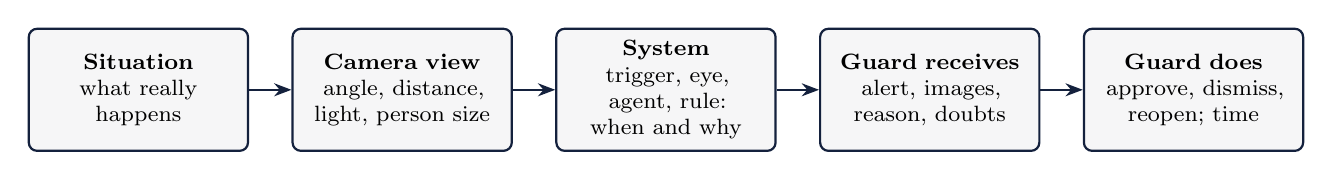
\begin{tikzpicture}[
  font=\footnotesize,
  sb/.style={draw=navy,thick,rounded corners=3pt,fill=navy!4,align=center,text width=2.55cm,minimum height=1.55cm},
  arr/.style={-{Stealth[length=2.2mm]},thick,draw=navy}]
\node[sb] (a) at (0,0) {\textbf{Situation}\\what really happens};
\node[sb] (b) at (3.35,0) {\textbf{Camera view}\\angle, distance, light, person size};
\node[sb] (c) at (6.7,0) {\textbf{System}\\trigger, eye, agent, rule: when and why};
\node[sb] (d) at (10.05,0) {\textbf{Guard receives}\\alert, images, reason, doubts};
\node[sb] (e) at (13.4,0) {\textbf{Guard does}\\approve, dismiss, reopen; time};
\draw[arr] (a)--(b); \draw[arr] (b)--(c); \draw[arr] (c)--(d); \draw[arr] (d)--(e);
\end{tikzpicture}
\end{center}

\begin{keybox}
\textbf{The demo that shows the idea: same footage, two sites.} A person walks along a corridor at 02:00. With a
hospital profile, this is routine. With a closed-office profile, it is a level-2 alert with its reason. Only the site
knowledge changed. The agent layer already shows the reverse case: the cleaners and the guard's car were dismissed
because the roster and badge log explained them.
\end{keybox}

\section{Who owns what}
Workstreams follow the member roles of the agent-layer check-in; owners are confirmed in Decision~D.

\begin{center}
\small
\begin{tabularx}{\textwidth}{L{3.6cm}YL{2.4cm}}
\toprule
\textbf{Workstream} & \textbf{Delivers} & \textbf{Owner}\\
\midrule
Data & Datasets, labels converted to events, a mostly-false site, blocked-exit and fire clips & Member 1\\
Perception: trigger & Motion and zone filter, detector, zones per camera, output format & Member 2\\
Perception: general eye & Open-vocabulary prompt, cascade, close look, image input (zoom, resolution) & to confirm\\
Search & Search index (Marengo), investigator agent, time to evidence & Member 3\\
Agent layer & Triage agent, site knowledge, rules, approval, reports, audit log & Member 4\\
Evaluation & Replay harness, frozen KPI runs, never-seen sites & shared\\
\bottomrule
\end{tabularx}
\end{center}

\section{Plan to 16 December}
Three weeks: we commit to the full chain on a small, honest scale, and keep the rest as stretch goals.

\begin{center}
\small
\begin{tabularx}{\textwidth}{L{1.5cm}Y}
\toprule
\textbf{By} & \textbf{Result}\\
\midrule
2 Dec & Decisions A--G taken. One KPI set frozen. Storyboards for the families. Eye models compared on the same clips (Gemini and Claude cascade). Datasets downloaded, labels converted to events. Site profile format fixed.\\
9 Dec & One pipeline: trigger $\rightarrow$ eye $\rightarrow$ triage agent $\rightarrow$ rules $\rightarrow$ guard, on the replayed MEVA site with a real (not stand-in) trigger. Eye with wider vocabulary. Site profile for a second site. First runs on 2 sites per family.\\
16 Dec & Results on never-seen sites, with and without site knowledge, KPIs 1--6 and 11. Demo: same footage, two sites.\\
\bottomrule
\end{tabularx}
\end{center}

\textbf{Committed:} person on the floor, object left, presence out of place, plus fire or violence if Decision~A
says yes; a site profile filled in by hand; at least one never-seen site.
\textbf{Stretch:} learned normal, investigator agent and time to evidence, report timing against writing by hand,
override rate after feedback, anonymous tracking, multi-camera views of one scene.
\textbf{Out of scope:} live streaming in production, identifying people, real actions (doors, calls), training our
own vision model.

\section{Decisions for the group}
\begin{description}[leftmargin=1.6em,labelwidth=1.2em,font=\bfseries\color{accent}]
\item[A.] Event families: accept the table in Section~4, including physical violence (facts only)?
\item[B.] Datasets in scope for 16 December (proposal in Section~6).
\item[C.] Site profile: fields of Section~5, filled in by hand; learned normal only if time allows?
\item[D.] Owners of the workstreams in Section~8, in particular the general eye.
\item[E.] The twelve KPIs and their targets (Section~6).
\item[F.] Models per role: which model for the first look, the second look and the triage agent? Proposal: decide
from one shared comparison on the same clips by 2 December, on accuracy per family, cost and time.
\item[G.] Anonymous tracking: pseudonyms inside one camera's footage only; linking people across cameras needs a
separate decision and a privacy note.
\end{description}

\vspace{0.5em}
{\footnotesize\color{gray}\textbf{About the numbers.} They come from two check-ins of 25 November and use small sets
(16 CAVIAR clips; 18 test clips and one 17-alert site). The agent layer's cascade rule was set after seeing its test
clips, and its detector knows the labels, so new clips and a real trigger must confirm both. Code: our main
repository and branch \texttt{cctv-playground}.\par}

\end{document}
